%%%%%%%%%%%%%%%%%%%%%%%%%%%%%%%%%%%%%%
% This is the name of the style file.
%%%%%%%%%%%%%%%%%%%%%%%%%%%%%%%%%%%%%%
%
% phd  -> for a PhD dissertation
% ms   -> for an MS thesis
% If both phd and ms are used then phd will overide.  If none are used,
% then ms will be active by default.
%
% cpyr -> generate a copyright page
% lof  -> generate List of Figures
% lot  -> generate List of Tables
\documentclass[ms,cpyr,lof,lot]{uathesis}
%
%%%%%%%%%%%%%%%%%%%%%%%%%%%%%%%%
% List of any packages you use.
%%%%%%%%%%%%%%%%%%%%%%%%%%%%%%%%
%

%% FROM REU SUMMARY


\usepackage{graphicx}
\usepackage{amsmath,amssymb}
%\usepackage{gensymb}
\usepackage{mathtools}
\usepackage{etoolbox}
\usepackage{booktabs}
\usepackage{float}
\usepackage{graphicx}
\usepackage{geometry}
\usepackage{multicol}
\usepackage{caption}
\usepackage[outdir=./eps2pdf/]{epstopdf}
\graphicspath{
  {figures/}
  {figures/goals/}
  {figures/light_data/}
  {figures/attenuation/}
}

%%%%%%%%%%%%%%%%%%%%%%%%%%%%%%%%%%
% List of definitions you define.
%%%%%%%%%%%%%%%%%%%%%%%%%%%%%%%%%%


\DeclareMathOperator{\atantwo}{atan2}


%% FROM GOALS
\newcommand\plotwidth{7in}

%% FROM REU SUMMARY

\newcommand{\ds}{\displaystyle}

% Define error function for math mode
\newcommand{\erf}{\mbox{erf}}
% Sign function
\newcommand{\sign}{\mbox{sign}}
% Real numbers
\newcommand\R{\mathbb{R}}
% Norm
\newcommand\norm[1]{||#1||}
% Length matrix entries
\newcommand\LL{\mathcal{L}}
% Frond population
\newcommand\FF{\mathcal{F}}

%% FROM RTE PAPER

% Natural numbers
\newcommand\NN{\mathbb{N}}
% Real numbers
\newcommand\RR{\mathbb{R}}
% Complex numbers
\newcommand\CC{\mathbb{C}}
% Curly B for basis
\newcommand\BB{\mathcal{B}}
% Curly D for diagonal dominance quantity
\newcommand\DD{\mathcal{D}}
\newcommand\QQ{\mathcal{Q}}
% Uniform Norm
\newcommand\unorm[1]{\left\lVert #1 \right\rVert_\infty}
% Inner Product
\newcommand\ip[1]{\left\langle #1 \right\rangle}
% Absolute value
\newcommand\abs[1]{\left| #1 \right|}
% Complex Conjugate
\newcommand\conj\overline
% Partial derivative
\newcommand\pd[2]{\frac{\partial #1}{\partial #2}}
% Iteration superscript w/ parentheses
\newcommand{\iter}[1]{^{(#1)}}
% Disable paragraph indentation
%\setlength{\parindent}{0pt}
% End of proof
\newcommand\qed{\hfill$\blacksquare$\hspace{0.5in}}


\title{Modelling the Radiation Field in Macroalgae Aquaculture}
\author{Oliver Graham Evans}
\conferraldate{May}{2018}

%The following commands specify the names and titles of people that
%will appear on the signature page.
%
%These four will always be needed.
\advisor{Dr. Kevin Kreider}
\chair{Dr. Kevin Kreider}
\collegedean{Dr. John Green}
\gradschdean{Dr. Chand Midha}
%
%For a PhD dissertation, specify a coadvisor and three committee
%members, or four committee members only.  For an MS thesis use either
%one coadvisor or one faculty reader, not both.
%
%Typical commands for a PhD dissertation (uncomment only 4).
%\coadvisor{Name of Coadvisor}
%\committee{Name of 1st Comm Member}
%\committee{Name of 2nd Comm Member}
%\committee{Name of 3rd Comm Member}
%\committee{Name of 4th Comm Member}
%
%Typical commands for an MS thesis (uncomment only 1).
\coadvisor{Dr. Curtis Clemons}
%\facreader{Name of Fac Reader}
%\facreader{Name of Fac Reader}

\begin{document}

\maketitle
\chapter{INTRODUCTION} \label{ch:intro}

\section{Purpose, Kelp \& WWTPs}
I spent this summer participating in an REU at Clarkson University developing a mathematical model for the light field in a macroalgae aquaculture environment. The impetus for this project was as follows: Dr. Rogers was approached by the operator of a wastewater treatment plant in Boothbay Harbor, Maine, who is facing increasingly demanding EPA regulations limiting the concentration of certain nutrients permissible to be released into the ocean via wastewater treatment outfalls.
In order to adhere to these stricter requirements using conventional nutrient remediation, a significant quantity of specialized equipment would be necessary, which is not currently present in the Boothbay Harbor plant.
Being surrounded on all sides by water and private property, the treatment plant lacks the necessary space for the additional equipment, and would therefore need to move their entire facility to a new location in order to conform to these new nutrient regulations.

As an alternative to conventional nutrient remediation techniques, Dr. Rogers has proposed the cultivation of the macroalgae \textit{Saccharina Latissima} (sugar kelp) near the outfall site.
The purpose of such an undertaking would be twofold: to prevent eutrophication of the surrounding ecosystem by sequestering the nutrients in question, and to reduce one of the primary expenses in macroalgae cultivation: nutrient input.
Once grown, a variety of products can be derived from macroalgae, including biofuel, fish/cattle feedstock, and high value chemical materials such as alginate and agar.
Food for human consumption is also a common product of kelp aquaculture, though it may not be ideal for a wastewater treatment application.

Thus, we seek to investigate the feasibility, and optimal implementation of kelp farming in wastewater treatment operations. 
Specifically, I seek to develop an accurate model of the light field in a kelp farming environment as a function of both the spacing and depth of the kelp plants, and of the quality of the water itself.
Ole Jacob Broch is a mathematician at SINTEF, a research organization in Trondheim, Norway, who has been working to model the growth of \textit{Saccharina Latissima} using SINMOD, a large-scale 3D hydrodynamical ocean model developed at SINTEF.
Ultimately, my aim is that my light model can be used both independently and in conjunction with Dr. Broch's SINMOD model.

\section{Background on Kelp Models}

Mathematical modeling of macroalgae growth is not a new topic, although it is a reemerging one.
Several authors in the second half of the twentieth century were interested in describing the growth and composition of the macroalgae \textit{Macrocystis pyrifera}, commonly known as ``giant kelp,'' which grows prolifically off the coast of southern California.
The very first such mathematical model was developed by W.J. North for the Kelp Habitat Improvement Project at the California Institute of Technology in 1968 using seven variables.
By 1974, Nick Anderson greatly expanded on North's work, and created the first comprehensive model of kelp growth which he programmed using FORTRAN \cite{anderson_mathematical_1974}.
In his model, he accounts for solar radiation intensity as a function of time of year and time of day, and refraction on the surface of the water.
He uses a simple model for shading, simply specifying a single parameter which determines the percentage of light which is allowed to pass through the kelp canopy floating on the surface of the water.
He also accounts for attenuation due to turbidity using Beer's Law.
Using this data on the availability of light, he calculates the photosynthesis rates and the growth experienced by the kelp. \\[-0.75em]

Over a decade later in 1987, G.A.
Jackson expanded on Anderson's model for \textit{Macrocystis pyrifera}, with an emphasis on including more environmental parameters and a more complete description of the growth and decay of the kelp \cite{jackson_modelling_1987}. 
He takes into account respiration, frond decay, and most importantly for my work, sub-canopy light attenuation due to self-shading.
He simply adds a coefficient to the exponential decay of light as a function of depth to represent shading from kelp fronds.
He doesn't seem to consider and radial nor angular dependence on shading.
Jackson also expands Anderson's definition of canopy shading, treating the canopy not as a single layer, but as 0, 1, or 2 discrete layers, each composed of individual fronds.
While this is a significant improvement over Anderson's light model, it is still rather simplistic. \\[-0.75em]

Both Anderson's and Jackson's model were carried out by numerically solving a system of differential equations over small time intervals.
In 1990, M.A. Burgman and V.A. Gerard developed a stochastic population model \cite{burgman_stage-structured_1990}.
This approach is quite different, and functions by dividing kelp plants into groups based on size and age, and generating random numbers to determine how the population distribution over these groups changes over time, based on measured rates of growth, death, decay, light availability, etc.
That same year, Nyman et. al. tested a similar model in New Zealand, as well as a Markov chain model, and compared the results with experimental data \cite{nyman_macrocystis_1990}. \\[-0.75em]

In 1996 and 1998 respectively, P. Duarte and J.G. Ferreira used the size-class approach to create a more general model of macroalgae growth, and Yoshimori et. al. created a differential equation model of \textit{Laminaria religiosa} with specific emphasis on temperature dependence of growth rate \cite{duarte_model_1997,yoshimori_mathematical_1998}.
These were the some of the first models of kelp growth that did not specifically relate to \textit{Macrocystis pyrifera} (``giant kelp''). 
Initially, there was a great deal of excitement about this species due to it's incredible size and growth rate, but difficulties in harvesting and negative environmental impacts have caused scientists to investigate other kelp species. \\[-0.75em]

In the last five years, a team at SINTEF, a research organization associated with the Norwegian University of Technology and Science (NTNU), based in Trondheim, Norway, has become interested in the aquaculture potential of the kelp \textit{Saccharina latissima} for use as food, animal feed, nutrient remediation, biofuel production, and high-value chemical production among other uses. 
In 2012, Ole Jacob Broch, whom I have been working with for the last few weeks, published a paper with Dag Slagstad describing the model they created of the growth and composition of \textit{S. latissima} over the course of the year \cite{broch_modelling_2012}.
Their model works in conjunction with SINMOD, a 3D hydrodynamic ecosystem model developed at SINTEF which generates data on water temperature, water velocity, light intensity, and phytoplankton concentrations among other valuable quantities \cite{wassmann_modelling_2006}.
This detailed information has allowed Ole Jacob to consider many factors which influence the growth and decay of kelp in greater detail than has previously been explored. \\[-0.75em]

The aspect of the model that he has asked me to help develop is how light is attenuated by kelp plants and by environmental factors, and how that affects the kelp's ability to photosynthesize and grow. 
This will allow us to estimate how deep and how densely kelp can be grown. This work is being done as a part of the MacroSea project, funded by the Norwegian Research Council, which intends to further develop the potential industrial kelp production through collaboration among industry and academia both in Norway and abroad. SINTEF and Clarkson are both involved in the project. \\[-0.75em]

In my model, I intend to combine the probabilistic aspects of models such as the one developed by \cite{burgman_stage-structured_1990} with numerically solving a system of differential equations such as is done by \cite{anderson_mathematical_1974} and \cite{broch_modelling_2012}
For example, the concept of a Lefkovitch model, which is essentially a Markov chain model which describes the change size distribution of a biological population which is broken up into discreet size classes, may prove to be very useful \cite{caswell_matrix_1983}. Combining the idea of a probabilistic model of shading based on the distribution of frond lengths and angles with differential equations describing the growth and decay of kelp fronds as a function of light availability may prove to be very powerful. I intend to analyze experimental data collected here in Norway, as well as in Maine and elsewhere in the literature to verify the model. \\[-0.75em]

\section{Background on Radiative Transfer}

We use monochromatic radiative transfer in order to model the light field in an aqueous environment populated by vegetation.
The vegetation (kelp) is modeled by a spatial probability distribution, which we assume to be given.
The two quantities we seek to compute are \textit{radiance} and \textit{irradiance}.
Radiance is the intensity of light in at a particular point in a particular direction, while irradiance is the total light intensity at a point in space, integrated over all angles.
The Radiative Transfer Equation is an integro-partial differential equation for radiance, which has been used primarily in stellar astrophysics; it's application to marine biology is fairly recent \cite{mobley_radiative_2001}.

We study various methods for solving the system of linear equations resulting from discretizing the Radiative Transfer Equation.
In particular, we consider direct methods, stationary iterative methods, and nonstationary iterative methods.
Numerical experiments are performed using Python's \texttt{scipy.sparse} \cite{jones_scipy:_2001} package for sparse linear algebra.
\texttt{IPython} \cite{perez_ipython:_2007} was used for interactive numerical experimentation.

Among those implemented, the nonstationary \texttt{LGMRES} \cite{baker_technique_2005} algorithm is the only algorithm determined to be suitable for this application without further work.
We discuss limitations and potential improvements, including preconditioning, alternative discretization, and reformulation of the RTE.

Understanding the growth rate and nutrient recovery by
kelp cultures has important marine biological implications. For example, recent
work by our research group at Clarkson University, the University of Maine, and
SINTEF Fisheries and Aquaculture is investigating kelp aquaculture as a means to
recover nutrients from wastewater effluent plumes in coastal environments into a
valuable biomass feedstock for many products. Current models for kelp growth
place little emphasis on the way in which nearby plants shade one another.
Self-shading may be a significant model feature, though, as light availability
may impact the growth and composition of the kelp biomass, and thus the mixture
of goods that may be derived.

\section{Summary of Main Results}
\chapter{MODEL DEVELOPMENT} \label{label:modeldevelopment}

\graphicspath{{./figures/}}

\section{General}

\section{Physical Setup}
Being a salt water species, macroalgae cultivation occurs primarily in the ocean, with the exception of the initial stage of growth, where microscopic kelp spores are inoculated onto a thread in a small laboratory pool.
This thread is then wrapped around a large rope, which is placed in the ocean and generally suspended by buoys in one of two configurations: horizontal or vertical.
Thus far, I am primarily concerned with modeling the vertical rope case, in which the kelp plants extend radially outward from the rope in all directions, which are made up of a single frond (leaf), stipe (stem) and holdfast (root structure).
We consider a rectangular grid of such vertical ropes. 
Plants extending from each rope will shade both themselves and their neighbors to varying degrees based on the depth of the kelp, the rope spacing, the angle of incident light and the nature of scattering in the water.
In addition, light will be naturally absorbed by the water to varying degrees as determined by the clarity of the water.

\begin{figure}[H]
	\centering
	\includegraphics[width=3.5in]{kelp_array}
	\captionof{figure}{$4\times 4$ array of vertical kelp ropes}
\end{figure}
\section{Coordinate System}
%For all of our three dimensional analysis, we will use the absolute coordinate system defined in figure \ref{fig:3dcoords}.
In the following sections, we will wish to convert between Cartesian and spherical coordinates, which we will do using the following formulas.
\begin{align}
	\begin{split}
		x & = r\sin\phi\cos\theta \\
		y & = r\sin\phi\sin\theta \\
		z & = r\cos\phi \\
	\label{eqn:coords}
	\end{split}
\end{align}

%Therefore, for some function $f(x,y,z)$, we can write its derivative along a path in spherical coordinates in terms of Cartesian coordinates using the chain rule.
\begin{equation}
	\frac{\partial f}{\partial r} 
	=\frac{\partial f}{\partial x}\frac{\partial x}{\partial r} 
	+ \frac{\partial f}{\partial y}\frac{\partial y}{\partial r} 
	+ \frac{\partial f}{\partial z}\frac{\partial z}{\partial r}
\end{equation}
Then, calculating derivatives from \eqref{eqn:coords}, we get
\begin{equation}
	\frac{\partial f}{\partial r} 
	=\frac{\partial f}{\partial x}r\sin\phi\cos\theta
	+ \frac{\partial f}{\partial y}r\sin\phi\sin\theta
	+ \frac{\partial f}{\partial z}r\cos\phi
	\label{eqn:partials}
\end{equation}
\begin{figure}[H]
	\centering
	\includegraphics[width=3in]{3d_coords}
	\caption{Downward-facing right-handed coordinate system with radial distance $r$ from the origin, distance $s$ from the $z$ axis, zenith angle $\phi$ and azimuthal angle $\theta$}
	\label{fig:3dcoords}
\end{figure}

\section{Kelp Model}

\section{2D Model}
First, let us consider a 2D vertical slab of width $dz$ of a single rope with kelp extending from it.
We assume that the number (not mass) density of kelp plants, $\rho$ is initially uniform along the length of the rope.

\subsection{Frond shape}
\label{sec:shape}

\begin{figure}[H]
	\centering
	\includegraphics[width=2in]{frond}
	\captionof{figure}{Model frond diagram}
	\label{fig:frond}
\end{figure}

The frond is a kite with length $l$ from base to tip, and width $w$ from left to right.
 %In figure \ref{fig:frond}, the base is shown at the bottom and the tip is shown at the top.
 The shortest distance from the base to the diagonal connecting the left and right corners is called $f_a$, and the shortest distance from that diagonal to the tip is called $f_b$.
 Clearly,
 \begin{equation}
	 f_a + f_b = l
 \end{equation}
When considering a whole population with varying sizes, it is more convent to specify ratios than absolute lengths.
Let the following ratios be defined.
\begin{align}
	f_r &= \frac{l}{w} \\
	f_s &= \frac{f_a}{f_b}
\end{align}
These ratios are assumed to be consistent among the entire population, making all fronds geometrically similar.
With these definitions, the shape of the frond can be fully specified by $l$, $f_r$, and $f_s$.
It is possible, then, to redefine $w$, $f_a$ and $f_b$ as follows from the preceding formulas.

\begin{align}
	w &= \frac{l}{f_r} \\
	f_a &= \frac{lf_s}{1+f_s} \\
	f_b &= \frac{l}{1+f_s}
\end{align}

The angle $\alpha$, half of the angle at the base corner, will be important in our analysis.
Using the above equations,
\begin{equation}
	\alpha = \tan^{-1}\left(\frac{2f_rf_s}{1+f_s}\right)
\end{equation}

\section{Population Distribution}
\label{sec:dist}

\subsection{Superindividuals}

The kelp lifecycle model of which this work is part is based on the concept of
superindividuals, which are kelp fronds which represent a subpopulation of
identical fronds.

** WE HAVE TO CALCULATE LENGTH BEFORE CALCULATING STANDARD DISTRIBUTION **

At each depth $k$, we have $n$ superindividuals, indexed by $i$. Superindividual
$i$ has a frond area $a_{ki}$ and represents $n_{ki}$ individual fronds.

\subsection{Length Distribution}

Given the superindividual data, we calculate the mean $\mu$ and standard deviation $\sigma$ frond
lengths using the formulas:
\begin{equation}
  \mu_k = \frac{\ds \sum_{i=1}^N a_{ki}}{\ds \sum_{i=1}^N n_{ki}} 
\end{equation}
\begin{equation}
  \sigma_k = \frac{\ds \sum_{i=1}^N \left( a_{ki} - \mu_k \right)^2}{\ds \sum_{i=1}^N n_{ki}} 
\end{equation}

We then assume that frond lengths are normally distributed in each depth layer
with mean $\mu_k$ and standard deviation $\sigma_k$.

\subsection{Frond angle distribution}
\label{sec:angle_dist}
The frond angle varies according to the von Mises distribution, which is the periodic analogue of the normal distribution.
It is defined on $[-\pi,\pi]$ rather than $(-\infty,\infty)$.
It has two parameters, $\mu$ and $\kappa$, which shift and sharpen the distribution respectively.
%$\kappa$ can be considered analogous to $1/\sigma$ in the normal distribution.
Here, we use $\mu = \theta_w$ and $\kappa = v_w$.

The PDF for this distribution is
\begin{equation}
	P_{\theta_f}(\theta_f) = \frac{e^{(v_w)\cos(\theta_f-v_w)}}{2\pi I_0(v_w)}
\end{equation}
where $I_0(x)$ is the modified Bessel function of the first kind of order 0.
Notice that unlike the normal distribution, the von Mises distribution approaches a \textit{non-zero} uniform distribution as $\kappa$ approaches 0.
\begin{equation}
	\displaystyle \lim_{v_w \to 0}P_{\theta_f}(\theta_f) = \frac{1}{2\pi} \;\forall\, \theta_f \in [-\pi,\pi]
\end{equation}
The idea behind using this distribution is that with zero current velocity, the frond angles should be distributed uniformly, while as current velocity increases, they should be increasingly likely to be pointing in the direction of the current.
Note that $\theta_w$ and $v_w$ are functions of position.
For a given depth layer, we will use the average water velocity for that depth.

\begin{figure}[H]
	\centering
	\includegraphics[width=\linewidth]{vonmises_2}
	\captionof{figure}{von Mises distribution for a variety of parameters}
	\label{fig:vonmises}
\end{figure}

\subsection{Combined 2D length-angle distribution}
\label{sec:2d_dist}
The previous two distributions are independent of one another. That is, the angle of the frond does not depend on the length, or vice versa.
Therefore, the probability of a frond simultaneously having a given frond length and angle is the product of their individual probabilities.

Given independent events $A$ and $B$,
\begin{equation}
	\label{eq:ind_prob}
	P(A \cap B) = P(A)P(B)
\end{equation}
Then the probability of frond length $l$ and frond angle $\theta_f$ coinciding is 
\begin{equation}
	P_{2D}(\theta_f,l) = P_{\theta_f}(\theta_f) \cdot L(l)
\end{equation}
A contour plot of this 2D distribution for a specific set of parameters is shown in figure \ref{fig:dist_2d}, where probability is represented by color in the 2D plane.
Darker green represents higher probability, while lighter beige represents lower probability.
In figure \ref{fig:kelp_sample}, 50 samples are drawn from this distribution and plotted.

It is important to note that if $P_{\theta_f}$ were dependent on $l$, the above definition of $P_{2D}$ would no longer be valid.
For example, it might be more realistic to say that larger fronds are less likely to bend towards the direction of the current.
In this case, \eqref{eq:ind_prob} would no longer hold, and it would be necessary to use the following more general relation.
\begin{equation}
	P(A \cap B) = P(A)P(B|A) = P(B)P(B|A)
\end{equation}
This is currently not taken into consideration in this model.

\begin{figure}[H]
	\centering
	\includegraphics[width=\linewidth]{prob_2d}
	\vspace{-3em}
	\captionof{figure}{2D length-angle probability distribution with $\theta_w=2\pi/3,v_w=1$}
	\label{fig:dist_2d}
\end{figure}

\begin{figure}[H]
	\centering
	\includegraphics[width=\linewidth]{kelp_sample}
	\vspace{-2em}
	\captionof{figure}{A sample of 50 kelp fronds with length and angle picked from the distribution above with $f_s=0.5$ and $f_r=2$.}
	\label{fig:kelp_sample}
\end{figure}

\subsection{Relative coordinate system}
\label{sec:rel_coords}
To determine under what conditions a frond will shade a given point, we begin by describing the shape of the frond in Cartesian and then polar coordinates.
Of primary interest are the edges connected to the frond tip.
For convenience, we will use a relative coordinate system $(\theta',s)$ such that the line connecting the base to the tip is vertical, with the base at $(0,0)$.
The Cartesian analogue of this coordinate system, $(x',y')$, has the following properties.
\begin{align}
	x' &= s\cos\theta' \\ 
	y' &= s\sin\theta'
\end{align}
and
\begin{align}
	s &= \sqrt{x'^2+y'^2}
\end{align}
\vspace{-1em}
\begin{align}
	\theta' &= \atantwo(y, x)
\end{align}

\subsection{Functional description of frond edge}
With this coordinate system established, we can describe the outer two edges of the frond in Cartesian coordinates as a piecewise linear function connecting the left corner: $(-w/2,f_a)$, the tip: $(0,l)$, and the right corner: $(w/2,f_a)$.
This function has the form
\begin{equation}
	y'_f(x') = l-\sign(x')\frac{f_b}{w/2}x'
\end{equation}
where
\begin{align}
	\sign(x) = 
	\begin{cases}
		1 & x > 0 \\
		0 & x = 0 \\
		-1 & x < 0 \\
	\end{cases}
\end{align}

%Using the equations in section \ref{sec:rel_coords}, this can be written in polar coordinates after some rearrangement as
\begin{equation}
	s_f'(\theta') = \frac{l}{\sin\theta' + S(\theta')\frac{2f_b}{w}\cos\theta'}
\end{equation}
where
\begin{equation}
	S(\theta') = \sign(\theta'-\pi/2)
\end{equation}

%Then, using the relationships in section \ref{sec:shape}, we can rewrite the above equation in terms of our frond ratios $f_s$ and $f_r$.
\begin{equation}
	\label{eq:rf_rel}
	s_f'(\theta') = \frac{l}{\sin\theta' + S(\theta')\frac{2f_r}{1+f_s}\cos\theta'}
\end{equation}

\subsection{Absolute coordinates}
\label{sec:abs_coords}
To generalize to a frond pointed at an angle $\theta_f$, we will use the coordinate system $(\theta,s)$ such that
\begin{equation}
	\theta = \theta' + \theta_f - \frac{\pi}{2}
\end{equation}
Then, for a frond pointed at the arbitrary angle $\theta_f$, the function for the outer edges can be written as 
\begin{equation}
	\label{eq:rf_abs}
	s_f(\theta) = s_f'\left(\theta - \theta_f + \frac{\pi}{2} \right)
\end{equation}


\subsection{Conditions for occupancy}
Consider a fixed frond of length $l$ at an angle $\theta_f$. The point
$(\theta,s)$ is occupied by the frond if
\begin{align}
	\left|\theta_f - \theta \right| < \alpha
	\shortintertext{and}
	s < s_f(\theta)
\end{align}

Equivalently, letting the point $(\theta,s)$ be fixed, a frond occupies the point if the following conditions are satisfied.
\begin{align}
	\theta - \alpha < \theta_f < \theta + \alpha
	\label{eqn:rs_th}
	\shortintertext{and}
	l > l_{min}(\theta,s)
	\label{eqn:rs_l}
\end{align}
where
\begin{equation}
	l_{min}(\theta,s) = s \cdot \frac{l}{s_f(\theta)}
\end{equation}


Then, considering the point to be fixed, \eqref{eqn:rs_th} and \eqref{eqn:rs_l} define the spacial region $R_s(\theta,s)$ called the ``occupancy region for $(\theta,s)$'' with the property that if the tip of a frond lies within this region (i.e. $(\theta_f,l) \in R_s(\theta,s)$), then it occupies the point.
$R_s(3\pi/4,3/2)$ is shown in blue in figure \ref{fig:shade_area} and the smallest possible occupying fronds for several values of $\theta_f$ are shown in various colors.
Any frond longer than these at the same angle will also occupy the point.

\begin{figure}[H]
	\centering
	\includegraphics[width=\linewidth]{shade_area}
	\vspace{-2em}
	\captionof{figure}{Outlines of minimum-length fronds for a variety of angles to occupy the point $(\theta,s)=(3\pi/4,3/2)$}
	\label{fig:shade_area}
\end{figure}

\subsection{Probability of occupancy}
NOT SO SURE ABOUT THIS
%We are interested in the probability that, given a fixed point $(\theta,s)$, values of $l$ and $\theta_f$ chosen from the distributions described in section \ref{sec:dist} will fall in the occupancy region.
%$This is found by integrating $P_{2D}$ over the occupancy region for $(\theta,s)$, as depicted in figure \ref{fig:cart_shade}.

\begin{figure}[H]
	\centering
	\includegraphics[width=\linewidth]{cart_shade}
	\vspace{-3em}
	\captionof{figure}{Contour plot of $P_{2D}(\theta_f,l)$ overlayed with the
    region in the $\theta_f-l$ plane which results in a frond occupying the point $(\theta,s)=(3\pi/4,3/2)$}
	\label{fig:cart_shade}
\end{figure}

Now, we are able to define the probability of a frond occupying the point $(\theta,s)$ at a depth $z$ at time $t$ by
\begin{align}
		P_k(\theta,s,z,t)	&= \iint_{R_s(\theta,s,z,t)}
								P_{2D}(\theta_f,l)
								\;dl\;d\theta_f \nonumber \\
							&= \int_{\theta-\alpha}^{\theta+\alpha} 
								\int_{l_{min}(\theta_f,z,t)}^\infty
								P_{2D}(\theta_f,l)
								\;dl\;d\theta_f
\end{align}

\begin{figure}[H]
	\centering
	\includegraphics[width=\linewidth]{prob_shade}
	\vspace{-2em}
	\captionof{figure}{Contour plot of the probability of occupying sampled at 121 points using $\theta_f=2\pi/3,v_w=1$}
	\label{fig:prob_shade}
\end{figure}


\section{Light Model}

\subsection{Background}
In terms of optical quantities, our primary interest is in the radiance at each point from all directions, which affects the photosynthetic rate of the kelp, and therefore the total amount of biomass producible in a given area as well as the total nutrient absorption potential.
The equation governing the radiance throughout the system is known as the Radiative Transfer Equation (RTE), which has been largely unutilized in the fields of oceanography and aquaculture.
Meanwhile, it has been studied extensively in two fields: stellar astrophysics and computer graphics.
In its full form, radiance is a function of 3 spatial dimensions, 2 angular dimensions, and frequency, making for an incredibly complex problem.
Thus far, I have ignored the dependence on frequency, and have only considered monochromatic radiation.
The RTE states that along a given path, radiance is decreased by absorption and scattering out of the path, while it is increased by emission and scattering into the path.
In our situation, emission is negligible, owing only perhaps to some small luminescent phytoplankton or some such anomaly, and can therefore be safely ignored.
\subsection{Optical Definitions}
One of the most fundamental quantities in optics is radiant flux $\Phi$, which is the has units of energy per time.
The quantity of primary interest in modeling the light field is radiance $R$, which is defined as the radiant flux per steradian per projected surface area perpendicular to the direction of propagation of the beam.
That is,
\begin{equation}
	R = \frac{d^2\Phi}{dA d\omega}
\end{equation}
We must now define a few inherent optical properties (IOPs) which depend only on the medium of propagation.

Consider a beam of light traveling through the water in the direction $\underline{\omega} = (\theta,\phi)$.
As it travels, there will be some decrease in the radiance due to scattering and absorption.
Let $a_w$ and $b_w$ be the coefficients of absorption and scattering respectively due solely to the water.
Similarly, define $a_k$ and $b_k$ to be the absorption and scattering coefficients due solely to kelp.
The loss due to scattering or absorption, whether by kelp or water, is proportional to radiance, and $a_w,b_w,a_k,b_k$ all have units of inverse meters.

There will also be some gain into the path of the beam due to scattering from other directions, as determined by the \textit{volume scattering function},
$\displaystyle \beta(\Delta\theta): [0,\pi) \rightarrow \R^+$, which gives the proportion of incident radiance scattered at an angle $\Delta\theta$ from its original direction due to only water.
The units of $\beta$ are $\mbox{m}^{-1}\mbox{rad}^{-2}$.

For convenience, let $\displaystyle \beta(\underline{\omega}_1,\underline{\omega}_2) = \beta\left(\cos^{-1}\left(\frac{\underline{\omega}_1\cdot\underline{\omega}_2}{\norm{\underline{\omega}_1}\norm{\underline{\omega}_1}}\right)\right)$. 

\subsection{PDE}
From the discussion above, our governing PDE, the radiative transfer equation, can be written as
\begin{equation}
	\frac{\partial R}{\partial r} = 
	- c_kP_k - (1-P_k)c_w
	+ \iint_{4\pi}
	\beta_k(\underline{\omega},\underline{\omega}')
	R(x,y,z,\underline{\omega}')\,d\underline{\omega}'
	\label{eqn:rte1}
\end{equation}
where $c_k = a_k + b_k$, $c_w = a_w + b_w$, and $\underline{\omega}' \neq \underline{\omega}$.

%Using \eqref{eqn:partials}, this can be rewritten in terms of Cartesian coordinates as
\begin{align}
	\begin{split}
	\frac{\partial R}{\partial x}\sin\phi \cos\theta 
	&+ \frac{\partial R}{\partial y}\sin\phi \sin\theta
	+ \frac{\partial R}{\partial z}\cos\phi \\ 
	&= - c_kP_k - (1-P_k)c_w \\
	&+ \iint_{4\pi}
	\beta_k(\underline{\omega},\underline{\omega}')
	R(x,y,z,\underline{\omega}')\,d\underline{\omega}'
	\end{split}
	\label{eqn:rte2}
\end{align}
\subsection{Boundary Conditions}
Though I have determined the PDE which governs the behavior of the radiance in the domain, I am lacking a full set of appropriate boundary conditions for the system.

Since we have one derivative per spatial dimension, we need one boundary condition per spatial dimension as well.
For $x$ and $y$, it may be favorable to use periodic boundary conditions in order to simulate a large array of kelp ropes spread out over the surface of the ocean.
It is worth mentioning, though, that special consideration may be necessary in order to account for smaller rope grids, for which edge effects neglected by periodic boundary conditions may become relevant.

It is the $z$ boundary condition which is puzzling me.
We should be able to make reasonable assumptions about the incident radiation from the atmosphere, though it seems that this is not sufficient.
We can only use atmospheric conditions for downwelling radiation.
It doesn't seem reasonable that radiance from above would have a direct effect on upwelling radiation.
In this sense, we only have half of the boundary condition that we need.
Then it seems that the other half should come from the bottom of the simulation.
But I would like to avoid putting any kind of specifically reflective or absorptive boundary on the \textit{bottom} of the simulation box, since the ocean would likely be much larger than the kelp.
In this case, it would be of interest to find some bottom boundary condition which allows for the free flow of radiance in and out of the bottom boundary.

\section{Irradiance and Flux}
Assume that the radiance $R_{ijklm}$ is known at all angles $(\theta_l,\phi_m)$ at all points $(x_i,y_j,z_k)$ on a Cartesian grid.
Since we seek to calculate the radiant flux $\Phi$ through each frond (i.e. the quantity of solar energy that it receives per unit time), we must first calculate the irradiance as an intermediate quantity.

\subsection{Formulation}
The downward irradiance $E$  at a point $(x,y,z)$ is defined as
\begin{align}
	E(x,y,z) &= \iint_{2\pi} R(x,y,z;\theta,\phi)\,d\theta d\phi.
\end{align}
Then
\begin{equation}
	E_{ijklm}= \sum_{\substack{l=1 \\ \theta_l < \pi/2}}^{M_\theta}\sum_{m=1}^{M_\phi} R_{ijklm}
\end{equation}

Let $F(\theta_f,l)$ be the 2D spatial region occupied by a frond of length $l$ pointed in the direction $\theta_f$.
\begin{equation}
	\Phi = \iint_{F(\theta_f,l} E(x,y,z)\,dxdy
\end{equation}

\subsubsection{Calculation}
Note that this region is kite shaped, which doesn't make for a straightforward analytical or numerical integral.
Thus, we introduce the transformation $\tau$ that maps a point $(u,v)$ on the unit square to the corresponding point $(x,y)$ on a vertical frond $F(\frac{\pi}{2},l)$
In particular, we have $\tau(-1,-1) = (0,0)$, $\tau(1,1) = (0,l)$, $\tau(1,-1) = (w/2,f_a)$, and $\tau(-1,1) = (-w/2,f_a)$.
In full, $\tau(u,v) = (x,y)$, where
\begin{align}
	x &= \frac{l(u-v)}{4f_r} \\
	y &= -\left(\frac{l}{4}\right) \frac{f_s(u-1)(v+1) - (u+1)(2f_s + v + 1)}{1+f_s}
\end{align}

The Jacobian of $\tau$, then, is given by
\begin{equation}
	J = \left(\frac{l}{16f_r}\right) \frac{u + v + 2 - f_s(u-1)(v-1)}{1+f_s} \\
\end{equation}

Note that we can generalize $\tau$ to map to a frond at any angle $\theta_f$ by introducing the 2D rotation matrix.
We can rotate a point $\underline{r}_1 = (x_1,y_1) \in \R^2$ to a new point $\underline{r}_2 = (x_2,y_2) \in \R^2$ by an angle $\theta$ about the origin by pre-multiplying by the rotation matrix $W_{\theta}$, where
\begin{equation}
	W_{\theta} = \left[ \begin{array}{cc}
		\cos\theta & -\sin\theta \\
		\sin\theta & \cos\theta \\
	\end{array} \right]
\end{equation}
That is
\begin{equation}
	\underline{r}_2 = W_{\theta} \underline{r}_1
\end{equation}

Let $T_{\theta} = W_{\theta} \tau$.
Then, $T_{\theta_f'}: [-1,1]\times[-1,1] \to F_{\theta_f}$ transforms $(u,v)$ on the unit square to the corresponding point $(x,y)$ on the frond with base at the origin pointing in the direction $\theta_f$

\subsubsection{Gaussian Quadrature}
With this in mind, we can use a Gaussian quadrature on the unit square to approximate the integral over the surface of a frond by summing the values for $E$ at the 4 points $\displaystyle\left\{T_{\theta_f'}\left(\pm\sqrt{\frac{1}{3}}\right)\right\}$. Although these points likely do not fall on our Cartesian grid for an arbitrary frond angle, we can use bilinear interpolation to approximate the value of $E$ at these points.
I have yet to study the efficiency and accuracy of this technique for calculating flux.

%%% FROM RTE 2D PAPER
\subsection{Radiative Transfer}
Let $n$ be the number of spatial dimensions for the problem (i.e., 2 or 3).
Let $x \in \RR^n$.
Let $\Omega$ be the unit sphere in $\RR^n$.
Let $\omega \in \Omega$ be a unit vector in $\RR^n$.
Let $L(x,\omega)$ denote \textit{radiance} position $x$ in the direction $\omega$.
Let $I(x)$ denote \textit{irradiance} at position $x$.
Let $P_k(x)$ be the probability density of kelp at position $x$.
Let $a_w$ and $a_k$ be the absorption coefficients of water and kelp respectively.
Let $b_w$ and $b_k$ be the scattering coefficients of water and kelp respectively.
Then we define the effective absorption and scattering coefficients as
\begin{align}
	\label{eq:abs}
	a(x) &= P_k(x) a_k + (1-P_k(x)) a_w \\
	\label{eq:sct}
	b(x) &= P_k(x) b_k + (1-P_k(x)) b_w
\end{align}
Then, the Monochromatic Time-Independent Radiative Transfer Equation (RTE) is
\begin{equation}
    \tag{RTE}
    \label{eq:rte}
    \begin{aligned}
        \omega \cdot \nabla_x L(x,\omega) &= -(a(x) + b(x)) L(x,\omega) \\
        &\qquad + b \int_\Omega \beta(\omega \cdot \omega') L(x,\omega')\, d\omega'
    \end{aligned}
\end{equation}

Note that in 2 spatial dimensions, this is a 3-dimensional problem ($x,y,\theta$).
Likewise, in 3 spatial dimensions, it is a 5-dimensional problem ($x,y,z,\theta,\phi$).

In this paper, we consider only the 2-dimensional problem, with the hope that sufficiently robust solution techniques for the 2-dimensional problem will be effective in the solution of the 3-dimensional problem as well.

\subsection{Boundary Conditions}
We assume that the downwelling light from the surface is known, and is defined to be uniform in space by the Dirichlet boundary condition
\begin{equation}
    L(x,0,\theta) = f(\theta), \quad \mbox{for} \quad \theta \in [0,\pi).
    \label{eq:surf_bc}
\end{equation}

Note that we cannot apply the same idea to upwelling light at the surface, as it cannot be specified from information about the atmospheric light field.
Therefore, we apply the PDE at $y=0$ for $\theta \in [\pi,2\pi)$.

At $y=1$, we assume no upwelling light.
That is,
\begin{equation}
    L(x,0,\theta) = 0, \quad \mbox{for} \quad \theta \in [\pi,2\pi).
    \label{eq:bottom_bc}
\end{equation}

As with the upper $y$-boundary, we apply the PDE for $\theta \in [0,\pi)$ so as not to prohibit downwelling light.

In the horizontal direction, we assume periodic boundary conditions.
Assuming that a single discrete group of plants is being simulated, adjusting the width of the domain effectively modifies the spacing between adjacent groups of plants.

\section{System of Linear Equations}

\subsection{Discretization}
In order to solve \eqref{eq:rte} numerically, we discretize the spatial derivatives using 2nd order finite difference approximations, and we discretize the integral according to the Legendre-Gauss quadrature, as described in \cite[Chapter 2]{chandrasekhar_radiative_1960}.
With this in mind, in order to create a spatial-angular grid with $n_x,n_y,
n_z, n_\theta$, and $n_\phi$ discrete values for $x, y, z, \theta$, and $\phi$
respectively, we use a uniform rectangular grid with spacings $dx = (x_{max} -
x_{min})/n_x$, etc. For the spatial variables, we have $x_i = x_{min} + (i-1) \cdot dx$
for $i=1,\ldots, n_x$. Then, $x_{n_x} = x_{max} - dx$.

Now, the angular grid requires a slight modification to account for the poles.
For $l = 1, \ldots, n_{\theta}$, $m = 2, \ldots, n_{\phi}-1$, we have
$(\theta_l, \phi_m)$ defined as before. Then, the values of variables at
$\phi=0, \phi=\pi$ are stored separately.

% Then, we have the grid
% \begin{align}
%     x_i &= (i-1)\,dx, &\quad i=1,\ldots,n_x \\
%     y_j &= (j-1)\,dy, &\quad j=1,\ldots,n_y \\
%     \theta_k \,\, \mbox{s.t.}\,\,
%     &P_{n_\theta}(\theta_k/\pi-1) = 0, &\quad k=1,\ldots,n_\theta
% \end{align}

In the same notational vein, let \\[-1em]
\begin{align}
    \beta_{kl} &= \beta(\abs{\theta_k-\theta_l}), \\
    a_{ij} &= a(x,y) \\
    b_{ij} &= b(x,y)
\end{align}

where $\abs{\cdot}$ is periodic as in \eqref{eq:rte}.

For the spatial interior of the domain, we use the 2nd order central difference formula (CD2) to approximate the derivatives, which is
\begin{equation}
    \tag{CD2}
    f'(x) = \frac{f(x+dx)-f(x-dx)}{2dx} + \mathcal{O}(dx^3).
\end{equation}

When applying the PDE on the upper or lower boundary, we use the forward and backward difference (FD2 and BD2) formulas respectively.
Omitting $\mathcal{O}(dx^3)$, we have
\begin{equation}
    \tag{FD2}
    \label{eq:FD2}
    f'(x) = \frac{-3f(x)+2f(x+dx)-f(x+2dx)}{2dx}
\end{equation}
\begin{equation}
    \tag{BD2}
    \label{eq:BD2}
    f'(x) = \frac{3f(x)-2f(x-dx)+f(x-2dx)}{2dx}
\end{equation}

As for the angular integral, we substitute a weighted finite sum of the function evaluated at the angular grid points.
For each $k$, let $a_k$ be the appropriate Legendre-Gauss weight according to \cite[Chapter 2]{chandrasekhar_radiative_1960}.
Then, applying the change of variables theorem to transform from the standard quadrature interval $[0,1]$ to the correct angular interval $[0,2\pi]$, we have
\begin{equation}
    \tag{LG}
    \int_0^{2\pi} f(\theta)\,d\theta \approx \pi\sum_{k=1}^n a_k f(\theta_k)
\end{equation}

\subsection{Difference Equation}
%Given the above discrete approximations, the difference equation for \eqref{eq:rte} in the spatial interior of the domain is
\begin{align}
    \label{eq:diffeq}
    \begin{split}
    0 &= \frac{1}{2dx}\left(L_{i+1,j}^k - L_{i-1,j}^k\right) \cos\theta_k
    - \pi b \sum_{\substack{l=1\\ l\neq k}}^{n_\theta} a_l\beta_{kl}L_{ij}^l \\
    &+ \frac{1}{2dy}\left(L_{i,j+1}^k - L_{i,j-1}^k\right) \sin\theta_k
    + (a_{ij} + b_{ij})L_{ij}^k
    \end{split}
\end{align}

%Similarly, we discretize using \eqref{eq:FD2} and \eqref{eq:BD2} at the boundaries.
For example, when $j=1$, we have
\begin{align}
    \label{eq:diffeq_bc}
    \begin{split}
    &\quad0 = \frac{1}{2dx}\left(L_{i+1,j}^k - L_{i-1,j}^k\right) \cos\theta_k
    - \pi b \sum_{\substack{l=1\\ l\neq k}}^{n_\theta} a_l\beta_{kl}L_{ij}^l \\
	&+ \frac{1}{2dy}\left(4L_{i,j+1}^k - L_{i,j+2}^k\right) \sin\theta_k
	+ (a_{ij} + b_{ij} -\frac{3}{2dy})L_{ij}^k
    \end{split}
\end{align}

Note that when discretizing the integral, we exclude the $l=k$ term of the sum.
This is because that term corresponds to ``scattering'' straight ahead ($\Delta\theta=0$), which is in fact not scattering at all.
Whether some adjustment to the quadrature is necessary to account for this is unclear.

\subsection{Structure of Linear System}
For each $(i,j,k)$, we have a distinct equation with $4+n_\theta$ variables.
This corresponds to a sparse matrix equation $Ax=b$, each row having $4+n_\theta$ nonzero entries.
Note that $b$ is zero at each row except those which correspond to boundary conditions in $y$.

Each element in $x$ and $b$ correspond to a particular triple $(i,j,k)$, as are each row and column of the coefficient matrix $A$.
In some sense, when we create this linear system, we are unwrapping a 3-dimensional quantity (radiance) into a 1-dimensional vector (the solution, $x$).
Different orders in which the equations are listed can be chosen to generate equivalent systems, so long as the ordering is consistent in $A,b$, and $x$.

The most obvious way to order the equations is to do so via a triple \texttt{for} loop, which has the effect of creating blocks in the matrix corresponding to planes in $(x,y,\theta)$ space.
For example, if the equations are ordered such that the outer \texttt{for} loop is over $x$, and the inner two are over $y$ and $\theta$, then the first $(n_y n_\theta)$ rows of the matrix correspond to the equations for $i=1$.

By switching the order of the \texttt{for} loops, we can generate 6 equivalent matrix systems, each of which can be identified with a permutation of the triple $(0,1,2)$, where 0 corresponds to $x$, 1 corresponds to $y$, and 2 corresponds to $\theta$, and the order of the numbers indicates the order in which the loops were nested, from outer to inner.

The coefficient matrices $A$, generated by each of these choices are shown below for a trivially small system with $n_x=n_y=n_\theta=6$.
Each black square represents a nonzero entry, whereas gray lines are purely for visual aid.

\pagebreak

\chapter{YOU NAME ANY CHAPTER HERE. MAKE SURE THEY'RE IN ALL CAPS} \label{lable_the_chapter_here}

This text is from the file chap4.tex.  Look at this file to see
the\footnote{Footnote text. Footnote text. Footnote text. Footnote
  text. Footnote text. Footnote text. Footnote text. Footnote text.
  Footnote text. Footnote text. Footnote text.}  format of this text.
A bibliography file will be need as well.  The bibliography file used
here is bio.bib.  Not this file as many entries but not all are used.
To reference a paper use $\backslash$cite{label}.  Here is a reference
for a paper \cite{Hagstrom_and_Hariharan}.  The book ASM
Handbook\footnote{Footnote text. Footnote text. Footnote text.
  Footnote text.}  Volume 15, \cite{Casting15}.

When running Latex you need two run the folling commands: \\
latex main.tex\\
latex main.tex\\
bibtex main\\
latex main.tex\\
latex main.tex\\
dvips -o main.ps main.dvi \\
Then you should have a postscript file you can read using ghost view (gv main.ps).
\ \\
{\em You will have problems, when you do look in a book, the web or ask someone.}



%%% Local Variables: 
%%% mode: latex
%%% TeX-master: t
%%% End: 

%\chapter{EXPERIMENTAL METHODS} \label{ch:experiment}

\section{Optical Properties}
\subsection{Absorption Coefficients}
\subsection{Scattering Coefficients}
\subsection{Volume Scattering Function}

\section{Frond Distribution Parameters}
\subsection{Rotation}
\subsection{Lift}

\section{Current Progress: Experimental Data Analysis}

\subsection{Experimental Setup}
Thus far, besides beginning to study literature on the subject, I have been analyzing data collected from an experiment that Dr. Rogers and his colleagues performed several weeks ago in the sea near Trondheim to measure attenuation with and without the influence of kelp shading. The experimental setup was as follows. A rope is attached to a buoy and allowed to hang freely in the water. Fixed to the rope are light sensors spaced 1m apart from one another from 1m below the water's surface to 8m. Samples are collected simultaneously from all sensors every 10 seconds for several hours. A second such rope is placed nearby in the water during the same time, but with one kelp plant attached to it. Similar measurements are taken. After a certain time, a second kelp plant is attached to the rope. Similar measurements are taken once again.

\subsection{Data and Model}
I was given raw data from the sensors separated into one text file for each light sensor, each containing many lines with the time and intensity of the individual measurements. I have used Python to perform some analysis on the data collected during the previously described experiment, and generate plots to visualize the data. I divided the raw data into 3 datasets:
\begin{itemize}
	\item \textbf{Control}: first rope without kelp,
	\item \textbf{1 Kelp}: second rope with one kelp plant
	\item \textbf{2 Kelp}: second rope with two kelp plants
\end{itemize}

Note that these datasets are not the same length. The sensors on the first rope were collecting data for a significantly longer period of time which encompassed the time periods when the other two datasets were being collected, as shown in the time plots below.

For each dataset, we sought to calculate the light attenuation according to the model:

\begin{equation}
	I(z) = I_0e^{-kz}
	\label{atten}
\end{equation}

where $I_0$ is the intensity of light on the surface of the water, and $k$ is the attenuation coefficient.

\pagebreak
\subsection{Regression Technique}
By doing exponential regression, these two parameters, $I_0$ and $k$ can be calculated. Notice that light is not actually being collected at the surface of the water, rather it is inferred based on the measurements at other depths.

These parameters can be calculated at each point in time in each dataset. This is done by converting the exponential model to a linear model by taking the logarithm of equation \ref{atten}, which gives

\begin{equation}
	\ln I(z) = \ln I_0 - kz
	\label{log_atten}
\end{equation}

Then, a simple least squares fit can be calculated by minimizing the sum, $R(k,I_0)$ of the squared differences between our linear model and the logarithm of the data points, given by the following function of our fit parameters.

\begin{equation}
	R(k,I_0) = \sum_{n=1}^N (\ln I_n - \ln I_0 + kz)^2
	\label{resid}
\end{equation}

where $z_n$ are the depths at which light is collected (i.e. 1m - 8m), $I_n$ are the measured intensities, and $N$ is the number of depths (i.e. 8). Let $R(k,I_0)$ be called the residual for the time step at we are performing the fitting. By taking partial derivatives with respect to both fit parameters, the residual can be minimized, producing the ideal fit (according to this definition of the residuals). Setting both derivatives to 0, we get the following matrix system of equations.

% Define x and y as used in this least squares fit
\newcommand\xls{z_n}
\newcommand\yls{\ln I_n}
\begin{equation}
	%\renewcommand\arraystretch{3}
	\begin{bmatrix}
		\sum_{n=1}^N \xls^2 & \sum_{n=1}^N \xls \\
		\sum_{n=1}^N \xls   & N \\
	\end{bmatrix}
%
	\begin{bmatrix}
		k \\
		I_0
	\end{bmatrix}
%
	=
%
	\begin{bmatrix}
		\sum_{n=1}^N \xls\yls \\
		\sum_{n=1}^N \yls \\
	\end{bmatrix}
	\label{lstsq}
\end{equation}

\subsection{Statistical Analysis}
\label{stats}
For each dataset, the previously described regression can be performed for each time step. This gives as many values of the fit parameters for the dataset as there are time steps. The mean ($\mu$) and standard deviation ($\sigma$) are given for both parameters for each dataset. Statistical description is also given of the $R^2$ values and of the raw intensity measurements (at all depths). \\

\begin{table}[H]
	\centering
	\begin{tabular}{lrrrr}
		\toprule
		&  $k$ & $I_0$ & Residuals & Intensity\\
		\midrule
		$\mu$ & 0.27 & 3.6+04 & 2.2e+09 & 1e+04 \\
		$\sigma$ & 0.046 & 2.7e+04 & 4.5e+09 & 1.3e+04 \\
	\end{tabular}
	\caption{Statistical info for \textbf{Control}}
	\label{stats_control}
\end{table}

\begin{table}[H]
	\centering
	\begin{tabular}{lrrrr}
		\toprule
		&  $k$ & $I_0$ & Residuals & Intensity\\
		\midrule
		$\mu$ & 0.34 & 5.6e+03 & 1.5e+09 & 2.2e+03 \\
		$\sigma$ & 0.25 & 2.1e+04 & 6.7e+09 & 1.3e+04 \\
	\end{tabular}
	\caption{Statistical info for \textbf{1 Kelp}}
	\label{stats_1_kelp}
\end{table}

\begin{table}[H]
	\centering
	\begin{tabular}{lrrrr}
		\toprule
		&  $k$ & $I_0$ & Residuals & Intensity\\
		\midrule
		$\mu$ & -0.65 & 3.4 & 2.9e+05 & 95 \\
		$\sigma$ & 0.12 & 4.3 & 5.2e+05 & 1.7e+02 \\
	\end{tabular}
	\caption{Statistical info for \textbf{2 Kelp}}
	\label{stats_2_kelp}
\end{table}
	
\pagebreak
\subsection{Visualization}
Several different visualization techniques are implemented below for the experimental data and for the fitted parameters

\subsubsection{Raw Data}

Light intensity is plotted over time for each of the 3 datasets. Each sensor is represented as a separate line.

\begin{figure}[H]
	\centering
	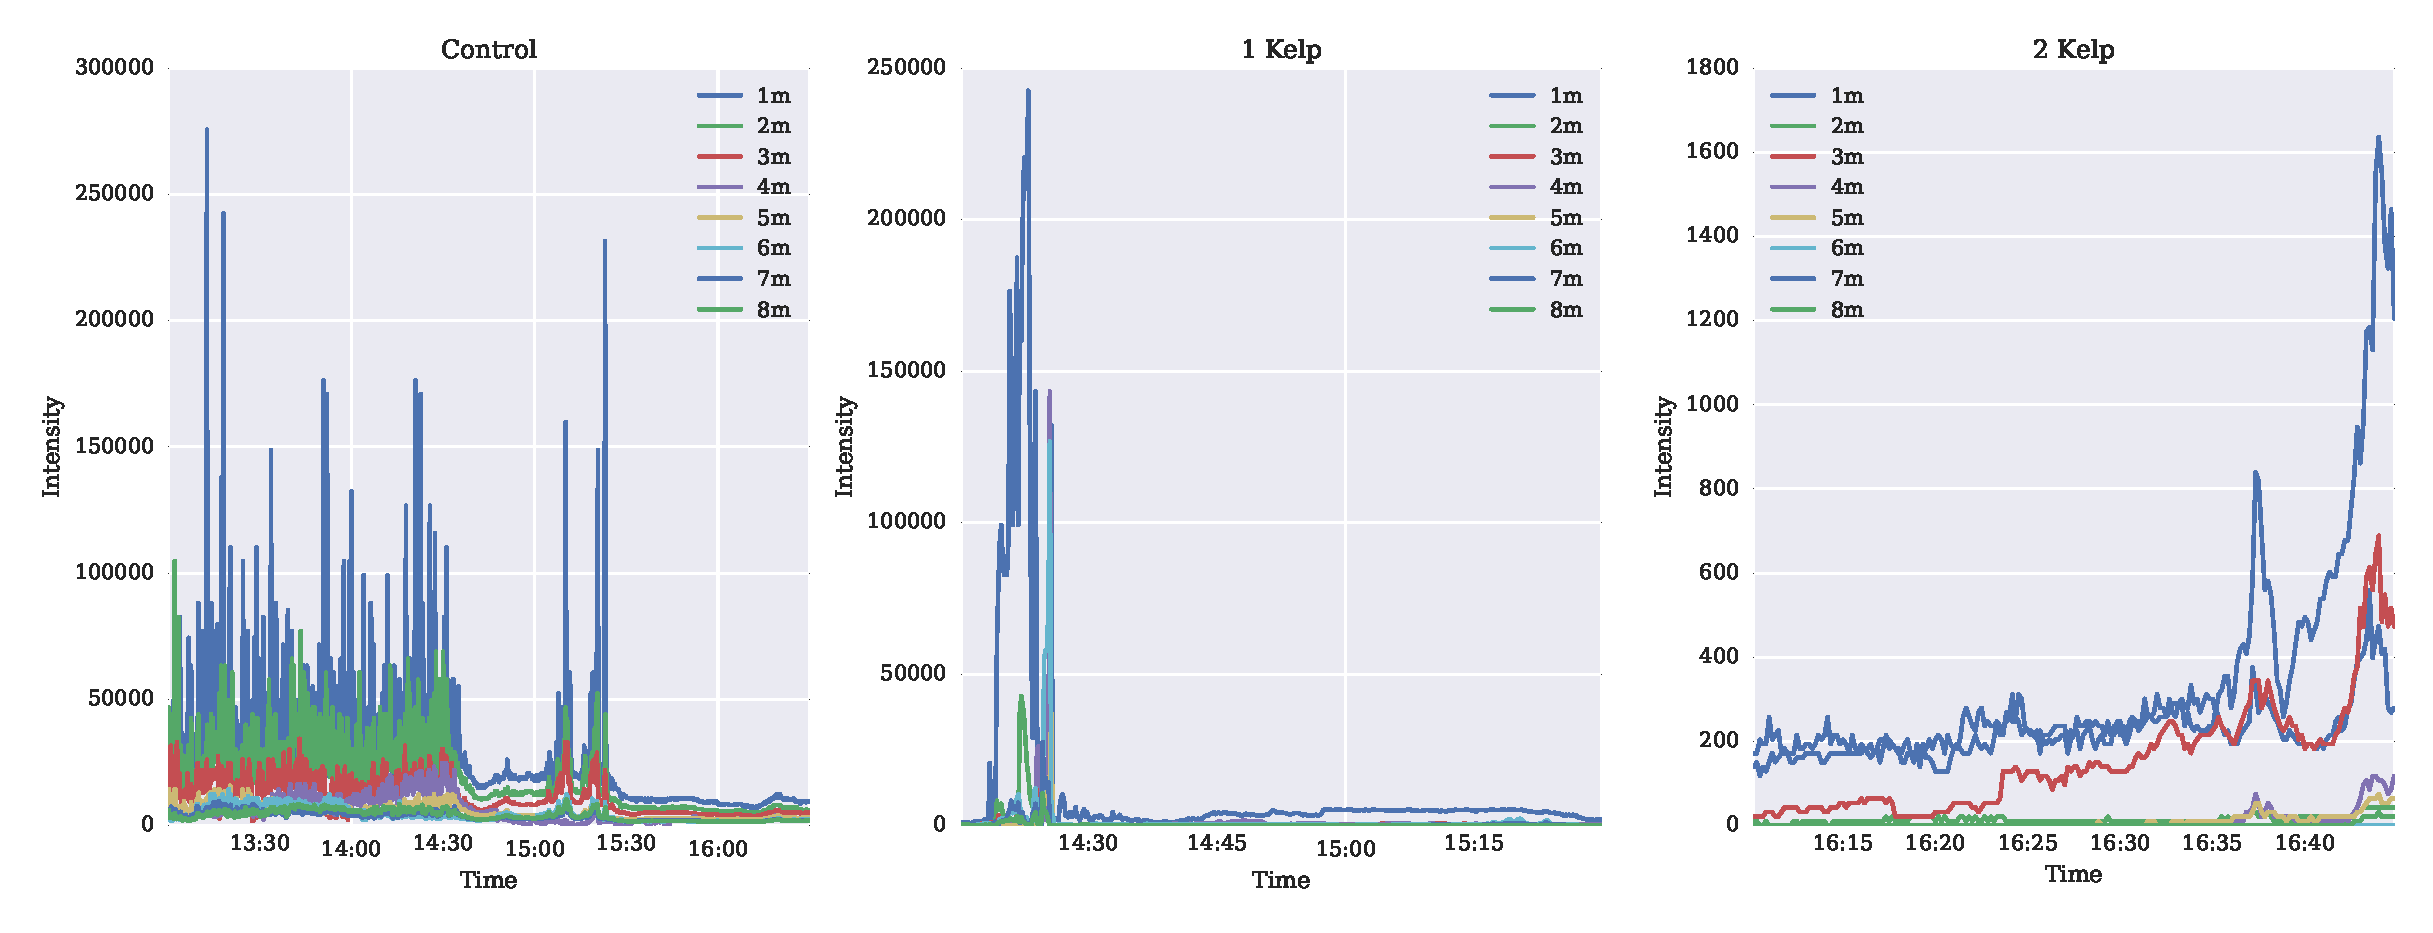
\includegraphics[width=\textwidth]{light_data.eps}
	\caption{Raw data: regular scale}
\end{figure}

\begin{figure}[H]
	\centering
	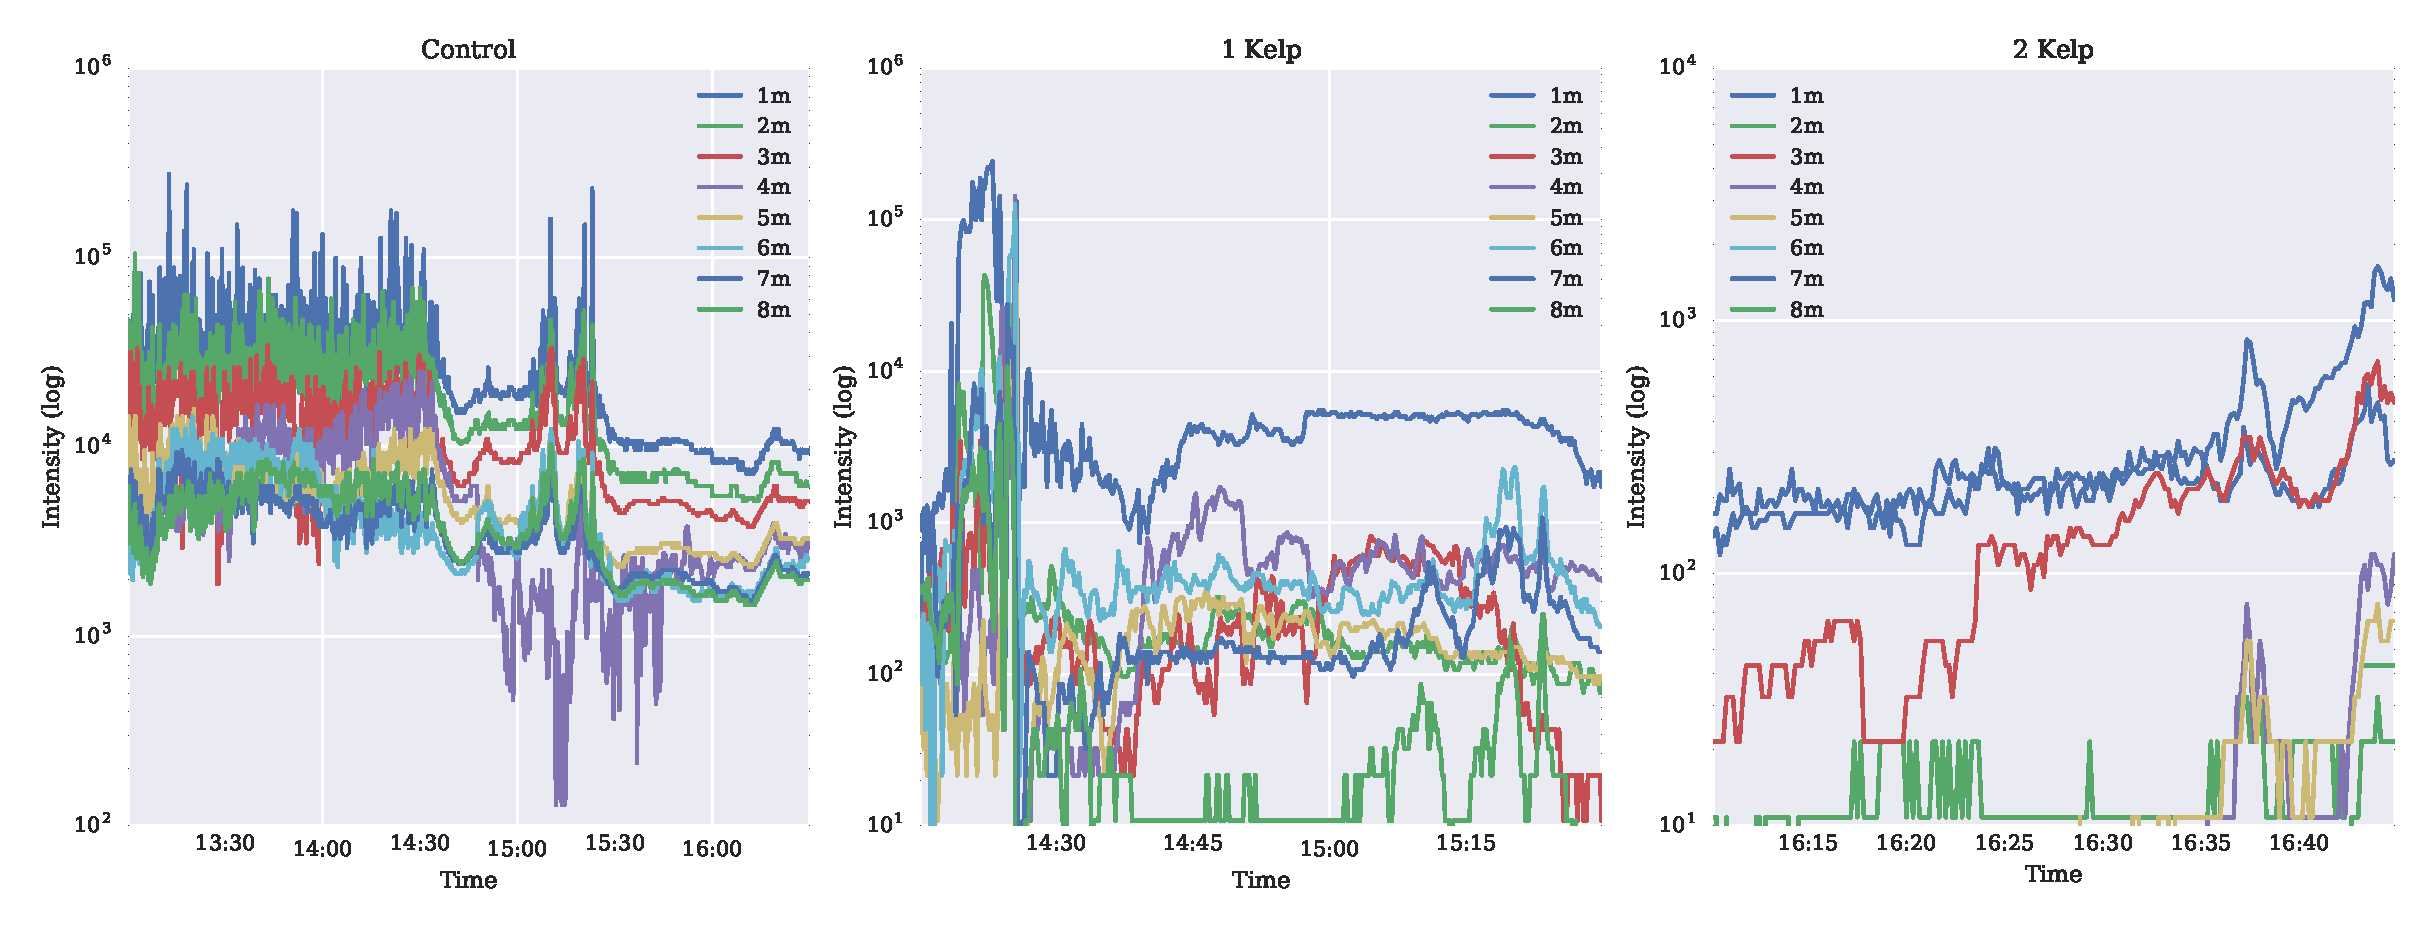
\includegraphics[width=\textwidth]{light_data_log.eps}
	\caption{Raw data: log scale}
\end{figure}

\pagebreak
\subsubsection{Parameters over time}
The fitted parameters are plotted over time. $R^2$ values are also plotted.

\begin{figure}[H]
	\centering
	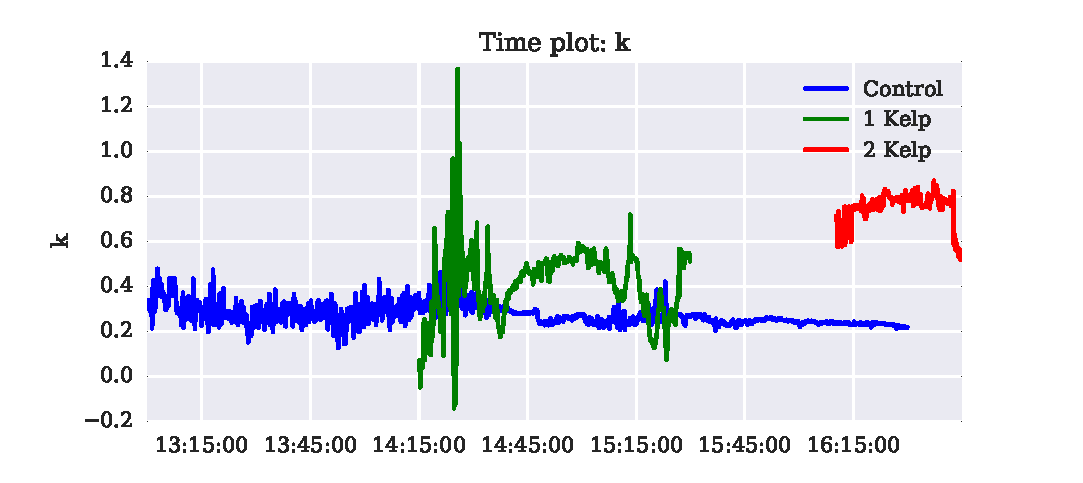
\includegraphics[width=\plotwidth]{time_k.eps}
	\caption{$k$ over time}
	\label{time_k}
\end{figure}

\begin{figure}[H]
	\centering
	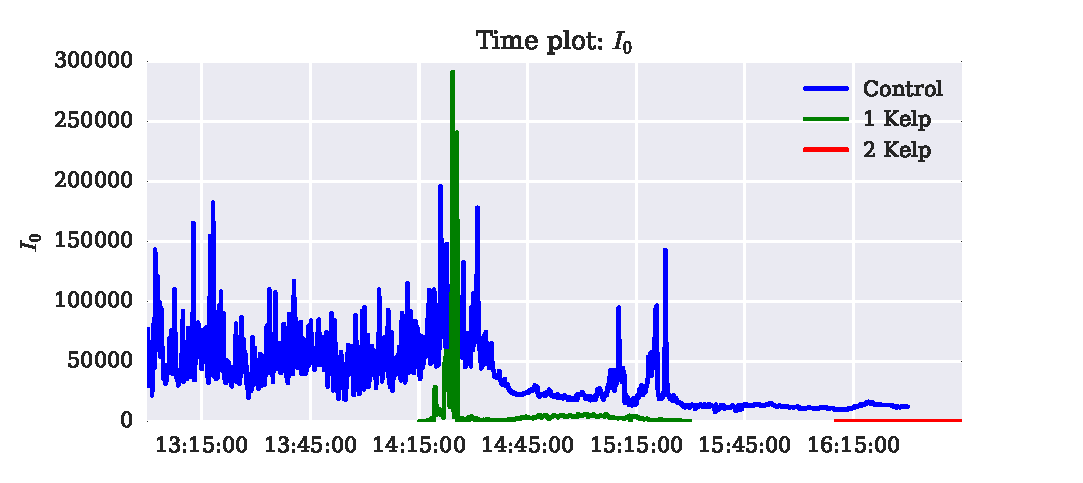
\includegraphics[width=\plotwidth]{time_I0.eps}
	\caption{$I_0$ over time}
	\label{time_I0}
\end{figure}

\begin{figure}[H]
	\centering
	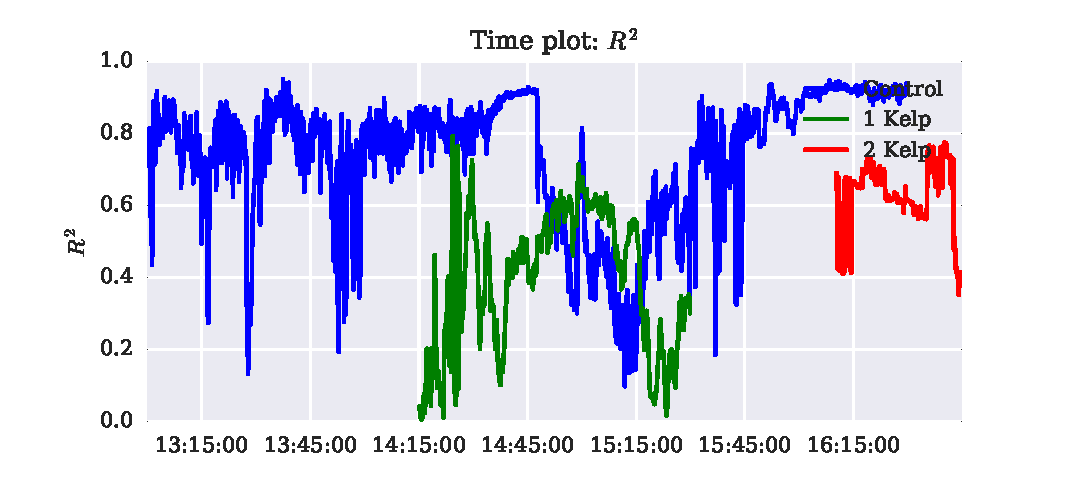
\includegraphics[width=\plotwidth]{time_r_squared.eps}
	\caption{$R^2$ over time}
	\label{time_r_squared}
\end{figure}

\subsubsection{Attenuation Coefficient Distribution}
The distributions of $k$ is shown using both bar plots and kernel density estimates (KDEs), in which each data point is represented by an exponential function of width similar to the bin width of the histogram, and the normalized sum of the exponentials is drawn to continuously represent the distribution.

\begin{figure}[H]
	\centering
	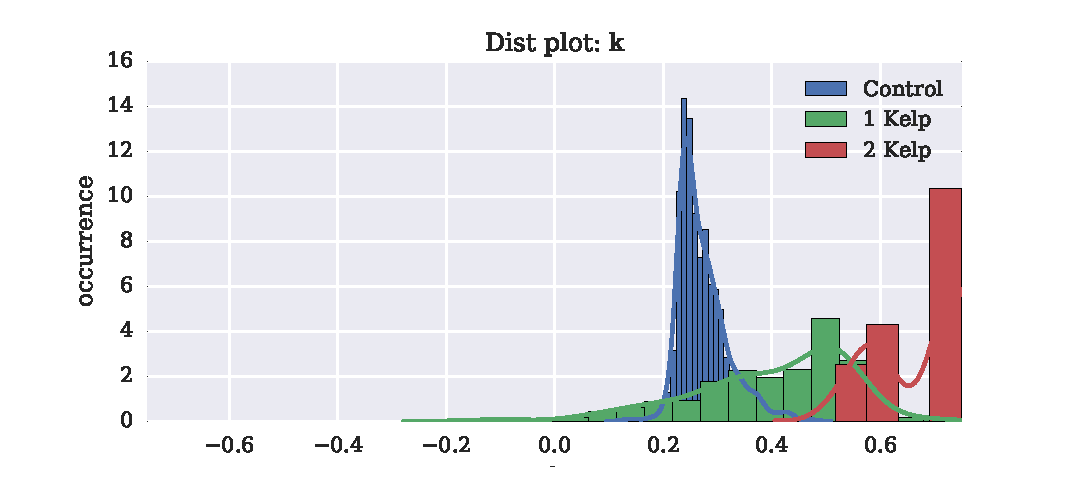
\includegraphics[width=\plotwidth]{dist_k.eps}
	\caption{Distribution of fitted values for attenuation coefficient}
\end{figure}

\subsubsection{Joint Plots}

The distributions of $k$ and $I_0$ are plotted together. In the first following figure, all three datasets are plotted together. In the following three plots, $k$ and $I_0$ are plotted using individual (1d) KDEs on the side and top, and a joint (2D) KDE represented by a contour plot in the center.

\begin{figure}[H]
	\centering
	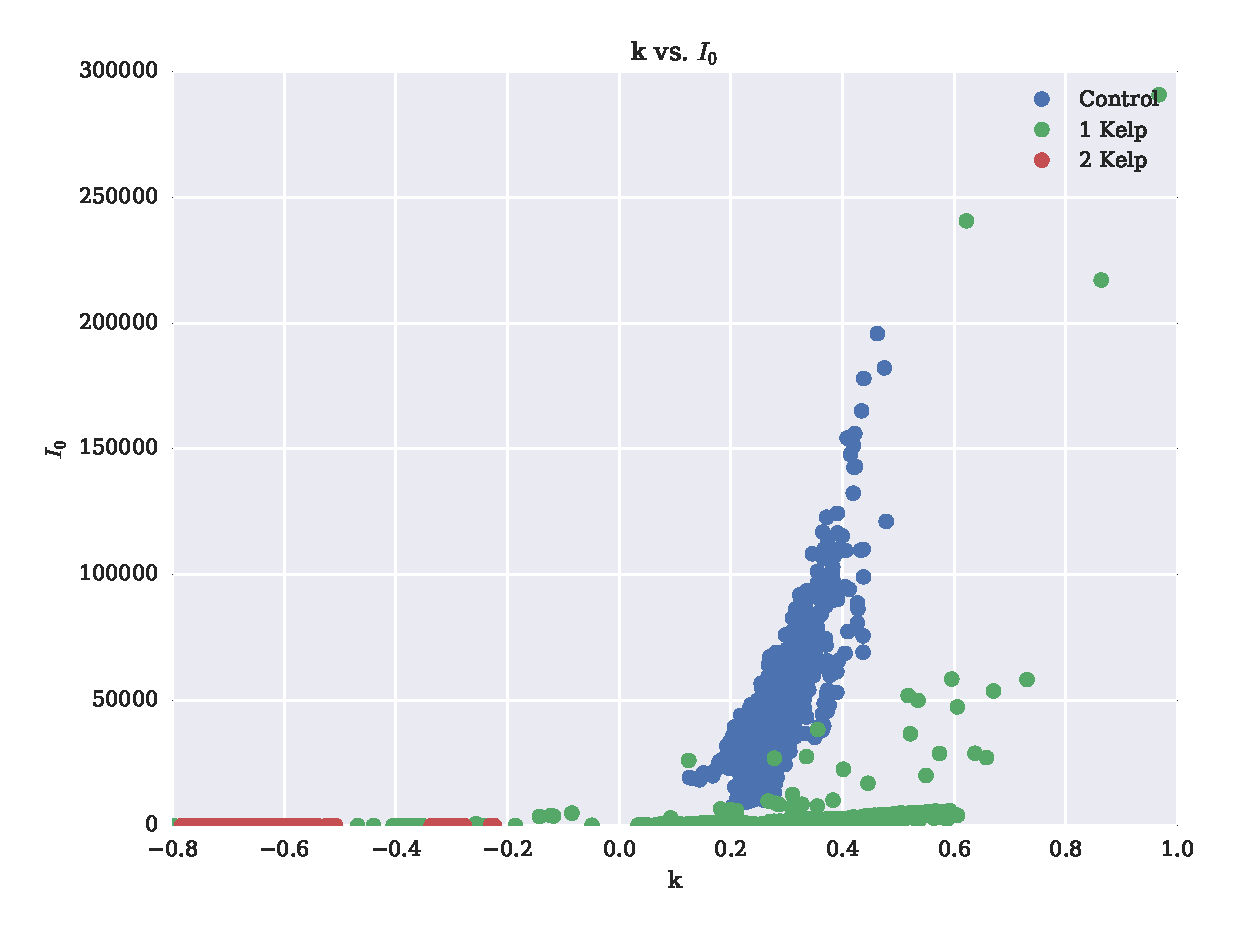
\includegraphics[width=\textwidth]{k_I0.eps}
	\caption{Joint distribution of $k$ and $I_0$ for all datasets}
\end{figure}

\begin{figure}[H]
	\centering
	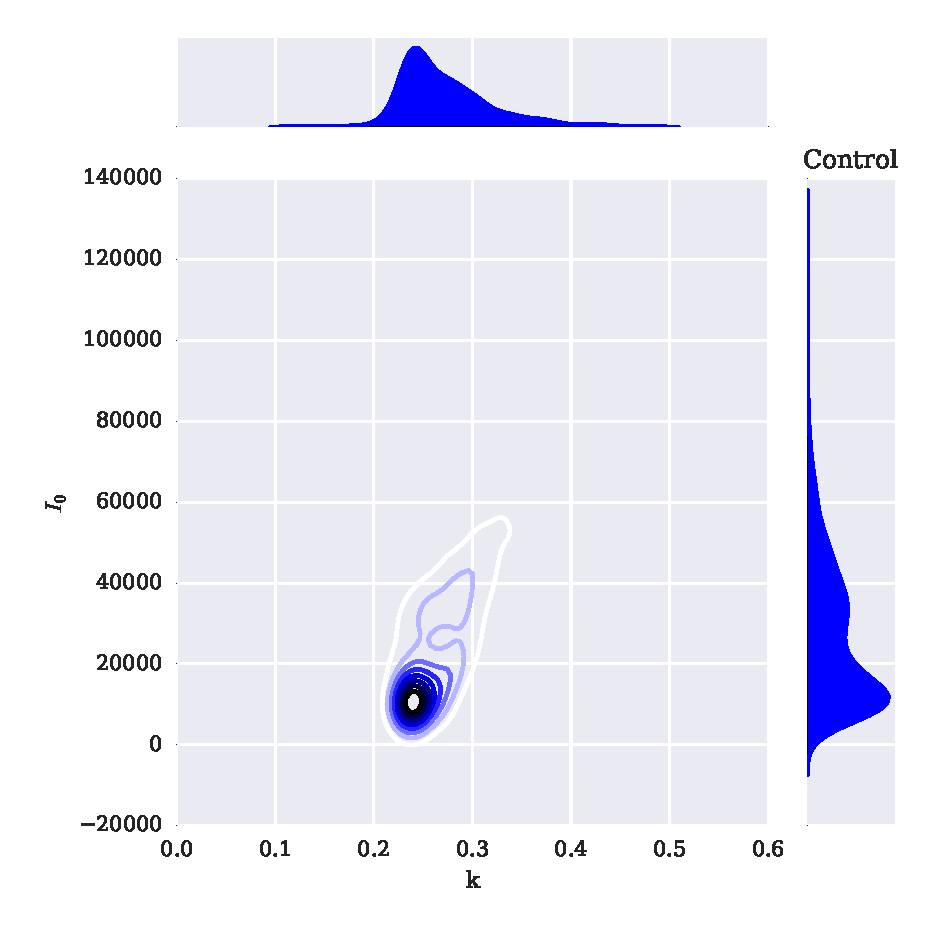
\includegraphics[width=\textwidth]{joint_control.eps}
	\caption{Joint distribution of $k$ and $I_0$ for \textbf{Control}}
	\label{joint_control}
\end{figure}

\begin{figure}[H]
	\centering
	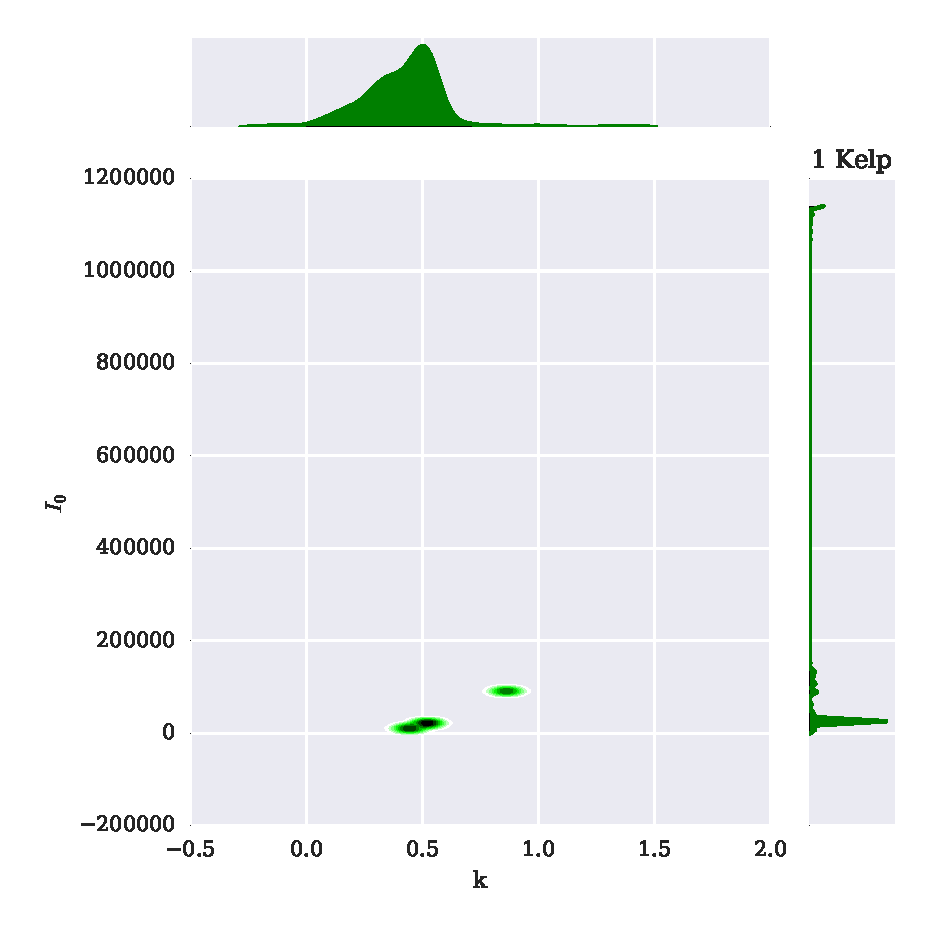
\includegraphics[width=\textwidth]{joint_1_kelp.eps}
	\caption{Joint distribution of $k$ and $I_0$ for \textbf{1 Kelp}}
	\label{joint_1_kelp}
\end{figure}

\begin{figure}[H]
	\centering
	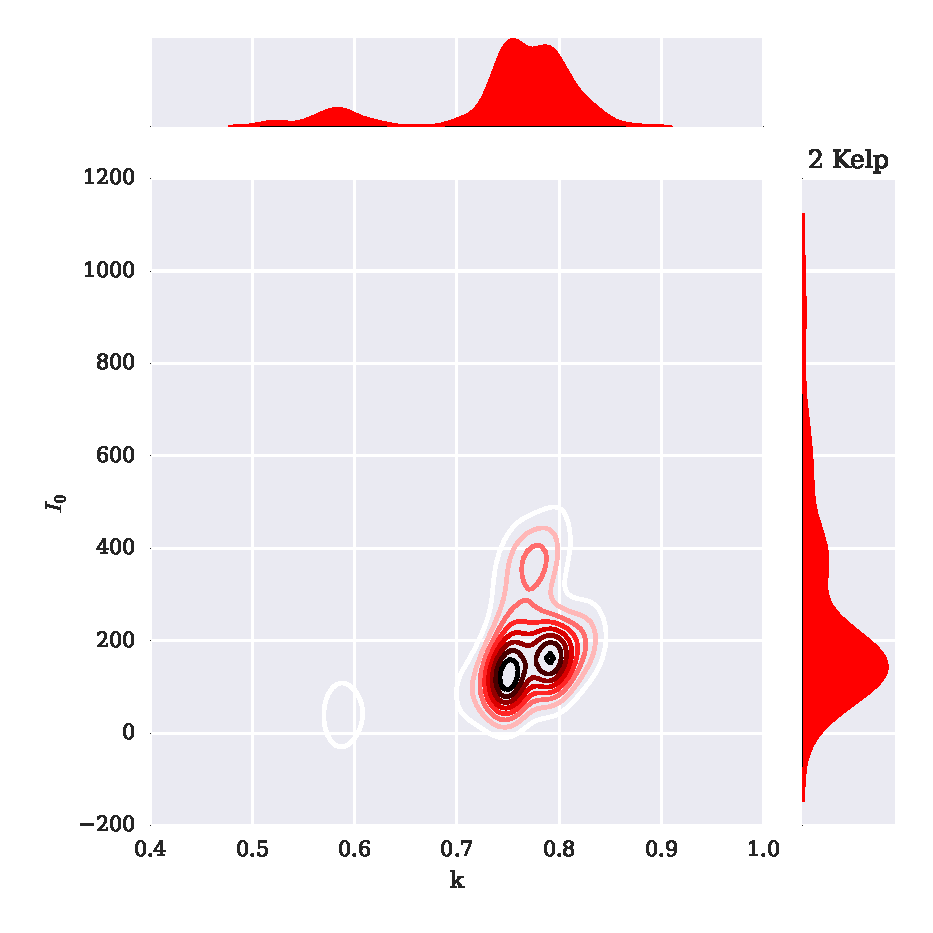
\includegraphics[width=\textwidth]{joint_2_kelp.eps}
	\caption{Joint distribution of $k$ and $I_0$ for \textbf{2 Kelp}}
	\label{joint_2_kelp}
\end{figure}

\subsection{Interpretation}
As is evident from the plots, all of the data is very noisy. The data does not fit the model perfectly, although in some cases the model is fairly successful. In particular, the attenuation measured by the sensors on the rope without kelp fits the model quite well, as can be seen by the relatively constant value for $k$ in figure \ref{time_k}, as well as by the small standard deviation shown in figure \ref{stats_control}. The model was fairly successful for the rope with 1 kelp plant. The data is certainly noisier than the control data. In figure \ref{joint_2_kelp}, it can be seen that the joint KDE for $k$ and $I_0$ seems to have 2 local maxima, which is symptomatic of a lack of consistency in the fitting. For the rope with 2 kelp plants, though, the analysis did not produce clear results. As is shown in the figures and the statistical table, negative values of $k$ are calculated. This would imply that light intensity is increasing with depth. Furthermore, the raw intensities as well as the calculated values for $I_0$ are several orders of magnitude lower than in the other cases. It is not clear why this is the case. Some possible cases are:
\begin{itemize}
	\item Kelp density varies with depth, so perhaps there is more kelp towards the surface than there is near the bottom of the rope.
	\item We are using the wrong time frame for this dataset. Perhaps the experiment with 2 kelp plants actually occurred at a different point during the day than the section being considered.
	\item The rope was placed in the water upside down. This could explain both the increasing intensity and lower magnitudes.
	\item Some unknown event was disrupting the experiment, e.g. large waves, fish, other boats, etc.
\end{itemize}

We will repeat the experiment on June 11th. Similar analysis will be performed with the new data, and the results will be compared.
\chapter{NUMERICS}
\section{Numerical Methods}

\section{Simulation Results}
\chapter{CONCLUSION}

% TODO: Write this
It was great and I've survived so far. Does future work go here?

\bibliographystyle{unsrt}
\bibliography{bio}
%If you have n appendices, then use the \appendices{n} command below
%followed by n \input{filename} commands, similar to the \input{chapx}
%commands above.
% DO NOT USE SECTIONS OR SUBSECTIONS IN AN APPENDIX OR APPENDICES
% \appendix{3}
% \chapter{APPENDIX TITLE GOES HERE} \label{ap:a}


{\bf DO NOT SECTION OR SUBSECTION AN APPENDIX OR APPENDICS}

We will recylcle Chapters~\ref{2DWaveEquation} and \ref{TabAndFigChap}
to make the following two appendices.


%%%%%%% DO NOT SECTION APPENDICES





% \chapter{SECOND APPENDIX: THE TWO DIMENSIONAL WAVE EQUATION} \label{ap:2DWaveEquation}

{\bf  DO NOT SECTION OR SUBSECTION AN APPENDIX OR APPENDICES}

A series solution for the two-dimensional wave equation
\begin{equation}
\frac{1}{c^{2}}\frac{\partial^{2}u}{\partial t^{2}} = \frac{\partial^{2}u}{\partial r^{2}} + %
        \frac{1}{r}\frac{\partial u}{\partial r} + \frac{1}{r^{2}}\frac{\partial^{2}u}%
        {\partial\theta^{2}}                                                                 \label{ap:waveEq}
\end{equation}
for outgoing waves is
\begin{equation}
u = \sum_{n=0}^{\infty}a_{n}(\theta)f^{n}(r,t),                                              \label{ap:Soln}
\end{equation}
where
\begin{equation}
f^{n} = \sum_{k=0}^{\infty}r^{-k-\frac{1}{2}}f_{k}^{n}(ct-r).                                \label{ap:function}
\end{equation} %look up reference.

You can reference a labeled equation by using the \textit{ref}
command.  For example, you can show that equations (\ref{ap:Soln}) and
(\ref{ap:function}) are a solution to equation (\ref{ap:waveEq}).
(see the file chap2.tex for the commands).



% \chapter{EXAMPLE OF A TABLE AND A FIGURE} \label{ap:TabAndFigChap}

{\bf DO NOT SECTION OR SUBSECTION AN APPENDIX OR APPENDICES}

\begin{table}[h]
\begin{center}
\caption{Table captions belong above the table} \label{ap:tb:disc}
\vskip .1 truein
\begin{tabular}{|l||c||c||c|} \hline \hline
\textbf{Name} & \textbf{Variable} & \textbf{Discretization} & \textbf{Step} \\ \hline
Radius      &       $r\in[a,R]$      &          $r_{k} =a + k dr,\quad k=0,1,2,\dots,K$   &    $dr = (R-a)/K$  \\ \hline
Angle       &       $\theta\in[0,2\pi)$ &      $\theta_{l} = l d\theta, \quad l =0,1,2,\dots,L-1$ & $d\theta = 2\pi/L$ \\ \hline
Time         &       $t\in[0,T]$           &      $t_{p} = p dt, \quad p =0,1,2,\dots,P$     &     $dt = T/P$ \\ \hline \hline
\end{tabular}
\end{center}
\end{table}

\begin{figure}[h]
\begin{center}
\includegraphics[width=3in,angle=-90]{Waves.eps}
\end{center}
\caption{Figure labels go below the figure} \label{ap:fg:N5Wave}
\end{figure}

To include figures side-by-side use the minipage environment.

\begin{figure}[ht]
\begin{minipage}{0.45\linewidth}
\begin{center}
\includegraphics[width=2.25in,angle=-90]{Waves.eps}
\vspace{0in}\ref{ap:sbys}A:
\end{center}
\end{minipage} \hfill
\begin{minipage}{0.45\linewidth}
\begin{center}
\includegraphics[width=2.25in,angle=-90]{Waves.eps}
\vspace{0in}\ref{ap:sbys}B:
\end{center}
\end{minipage}
\caption{Figures side-by side}\label{ap:sbys}
\end{figure}

See chap4.tex for the commands used to build the table and figure.  As
you add chapters, figures, and tables, the table of contents and lists
will automatically be updated.

Figure~\ref{ap:sbys} is an example of figures side-by-side, with
Figure~\ref{ap:sbys}A to the left of \ref{ap:sbys}B.


\end{document}
